\chapter{The Extensible Test Suite of Dresden OCL2 for Eclipse}
\label{chapter:generalTestSuite}

\begin{flushright}
\textit{Chapter written by Michael Thiele}
\end{flushright}

\acl{DOT4Eclipse} is a collection of Eclipse plug-ins that either are used together or some of these plug-ins are used together with plug-ins of other parties. This modular structure imposes one problem when trying to combine all test cases of \acl{DOT4Eclipse} into one test suite, since there is no guaranty that all test plug-ins are available.

Therefore, an extensible test suite has been created. It can be found under the name \reference{tudresden.ocl20.pivot.testsuite}. Basically it is a test suite that searches a specific extension point for registered tests or test suites. It includes these tests in its own test suite and executes the test suite. Thus, on any change of the source code all tests can be run at once to check the integrity of the toolkit.

To extend the extensible test suite with new tests or test suites, a plug-in has to implement the extension point \reference{tudresden.ocl20.pivot.testsuite}. This extension has to specify the tests it wants to add. JUnit3 as well as JUnit4 tests or test suites are allowed. If, for some reason, the test wants to emit some warnings to the user, it can use the Log4j mechanism for that purpose. Simply extend the \code{logger.properties} with the following code:
\code{# Extensible Test Suite appender
log4j.appender.stringbuffer=tudresden.ocl20.logging.appender.StringBufferAppender
log4j.appender.stringbuffer.layout = org.apache.log4j.PatternLayout
log4j.appender.stringbuffer.layout.ConversionPattern = \%C{1}: \%m\%n\%n}
Then add this appender to the logging of the plug-in. An example usage of this mechanism can be found in the plug-in \reference{tudresden.ocl20.pivot.metamodels.test}.

To run the extensible test suite, right-click on \code{OCL2TestSuiteRunner} in the package \code{tudresden.ocl20.pivot.testsuite.runner}. Choose \code{Run As} --\textgreater \code{JUnit Plug-in Test} as in figure \ref{pic:generalTestSuite:RunAs}.

\begin{figure}[!htbp]
	\centering
	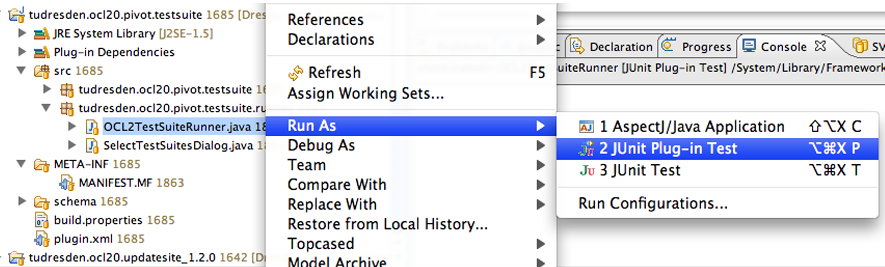
\includegraphics[width=1.0\linewidth]{figures/generalTestSuite/RunAs}
	\caption{Run the extensible test suite.}
	\label{pic: generalTestSuite:RunAs}
\end{figure}